\documentclass[12pt]{article}
\usepackage[utf8]{inputenc}
\usepackage[brazilian]{babel}
\usepackage{geometry}
\geometry{a4paper, total={170mm,250mm}, left=25mm, right=25mm, top=25mm}
\usepackage{graphicx}
\usepackage{titling}
\usepackage{float}
\usepackage{amsmath}

\title{Trabalho 2 - MEC2403 (Otimização)}
\author{Kleyton da Costa (2312730)}
\date{\today}
 
\usepackage{fancyhdr}
\fancypagestyle{plain}{%  the preset of fancyhdr 
    \fancyhf{} % clear all header and footer fields
    %\fancyfoot[R]{\includegraphics[width=3cm]{di.png}}
    \fancyfoot[L]{\today}
    \fancyhead[L]{Trabalho 2}
    \fancyhead[R]{\theauthor}
}
\makeatletter
\def\@maketitle{%
  \newpage
  \null
  \vskip 1em%
  \begin{center}%
  \let \footnote \thanks
    {\LARGE \@title \par}%
    \vskip 1em%
    %{\large \@date}%
  \end{center}%
  \par
  \vskip 1em}
\makeatother

\begin{document}

\maketitle

\noindent\begin{tabular}{@{}ll}
    Aluno & \theauthor \\
    Professor &  Ivan Menezes (MEC/PUC-Rio) \\
    Data & \today
\end{tabular}


\section{Introdução}

Este trabalho tem como objetivo implementar dois métodos indiretos de otimização com restrições: penalidade e barreira. Para alcançar este objetivo foram considerados dois métodos de otimização que servirão como entrada para os métodos com restrição, sendo eles o método de Powell e o BFGS.

\section{Metodologia}

Nesta seção iremos descrever brevemente os métodos de Penalidade e Barreira.

O método de penalidade pode ser utilizado para converter problemas de otimização com restrições em problemas sem restrições. Isso ocorre através da inserção de um termo de penalidade na função objetivo, permitindo que os métodos sem restrições possam ser utilizados: Univariante, Powell, Steepest Descent, BFGS, Flercher-Reeves e Newton-Raphson. 

Considerando o problema geral de otimização, dado por:

\begin{equation}
  \begin{aligned}
      \text{Minimizar:} \quad f(x) \\
      \text{S.t:}\quad g(x) \leq 0\\
      h(x)=0
  \end{aligned}
\end{equation}

\noindent em que $f(x)$ é a função objetivo e $g(x)$ e $h(x)$ são as restrições do problema.

A estratégia de penalidade tem como objetivo minimizar uma função $\phi$ com um parâmetro $\rho$ de tal maneira que a função objetivo seja minimizada com base nas restrições ajustada pela penalização. Neste caso, temos que

\begin{equation}
  \phi(x, \rho) = f(x) + \frac{1}{2}\rho p(x)
\end{equation}

\noindent em que $p(x)$ é a função penalidade.

Para o método da barreira a função $\phi$ é dada por 

\begin{equation}
  \phi(x, \rho) = f(x) + \rho \sum_{l=1}^{p}-\frac{1}{c_{l}(x)}
\end{equation}

Com isso, a solução do prolema se encontra na minimização da função $\phi$ com os métodos de otimização sem restrições já conhecidos.

\section{Resultados e discussão}

Esta seção apresenta os resultado encontrados através da aplicação dos métodos indiretos para otimização com restrições.

\subsection{Problema 1}

\begin{equation}
  \begin{aligned}
      \text{Minimizar:} \quad & f(x_1, x_2) = (x_1 - 2)^4 + (x_1 - 2x_2)^2 \\
      \text{S.t:} \quad & x_1^2 - x_2 \leq 0
  \end{aligned}
\end{equation}

Aplicando o método da \textbf{penalidade} para o problema proposto obtemos resultados para o método de Powell e para o método BFGS. Os gráficos abaixo apresentam as curvas de nível para a função objetivo e a linha para a penalidade (linha em verde). Além disso, é possível observar o ponto inicial e o ponto ótimo encontrado pelo algoritmo.

\begin{figure}[H]
  \centering
  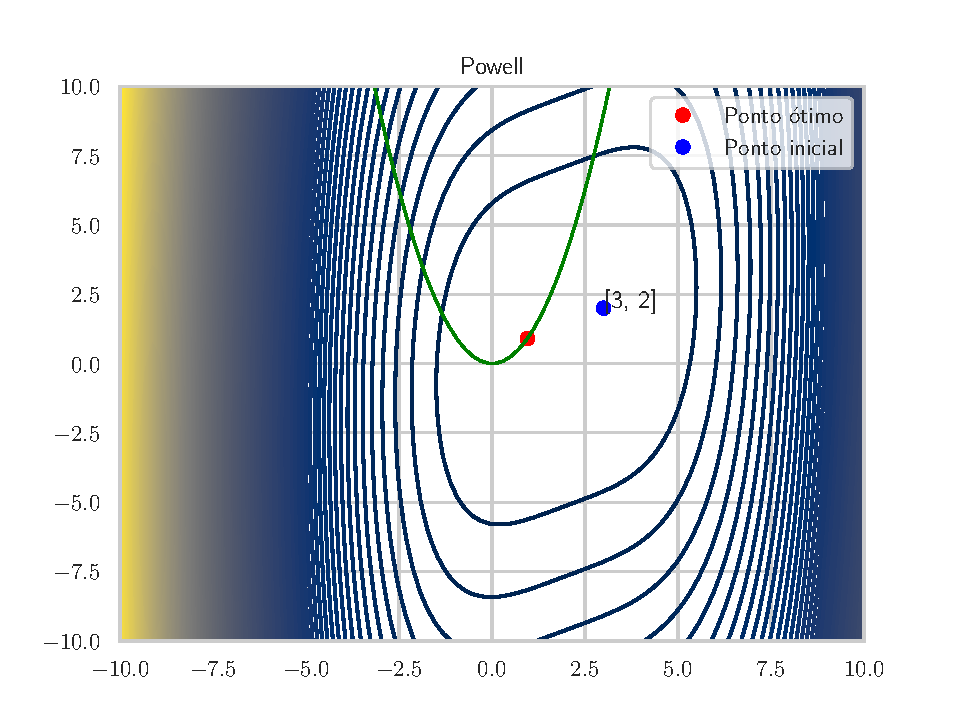
\includegraphics[scale = 0.6]{penalidade_Powell_[3 2].pdf}
\end{figure}

\begin{figure}[H]
  \centering
  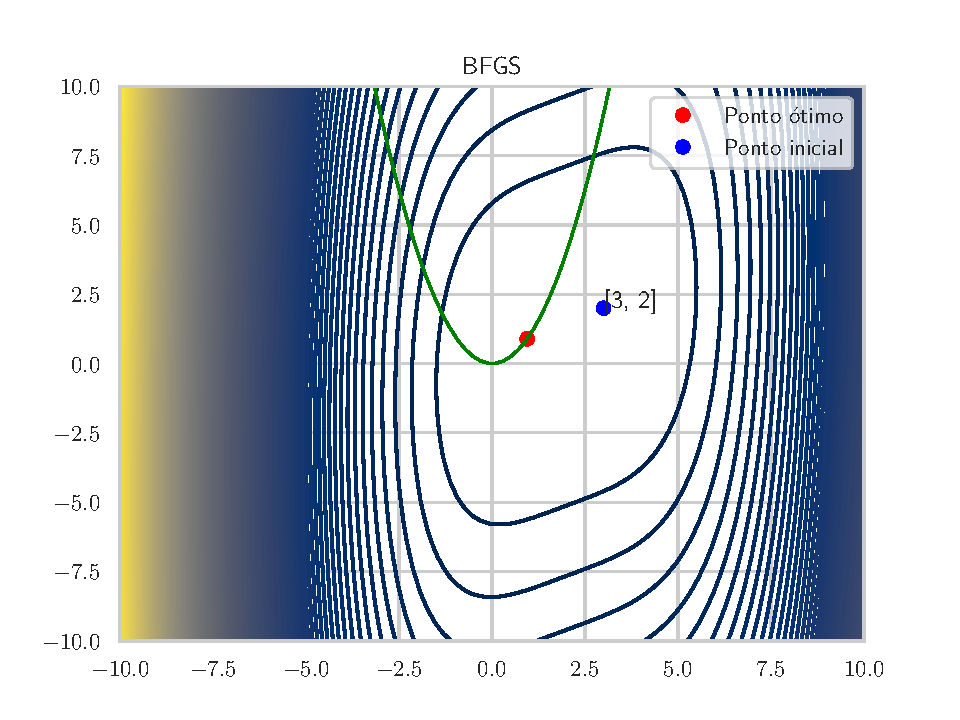
\includegraphics[scale = 0.6]{penalidade_BFGS_[3 2].pdf}
\end{figure}

A tabela abaixo mostra que os métodos obtiveram resultados próximos.

\begin{table}[H]
\centering
\begin{tabular}{llr}
  \hline
  Método & x & f(x) \\
  \hline
  Powell & [0.95017625 0.90283487] & 1.946560 \\
  BFGS & [0.94425484 0.89161819] & 1.946218 \\
  \hline
  \end{tabular}
\end{table}

Aplicando o método da \textbf{barreira} para o problema proposto obtemos resultados para o método de Powell e para o método BFGS. Os gráficos abaixo apresentam as curvas de nível para a função objetivo e a penalidade (linha em verde). Além disso, é possível observar o ponto inicial e o ponto ótimo encontrado pelo algoritmo.

\begin{figure}[H]
  \centering
  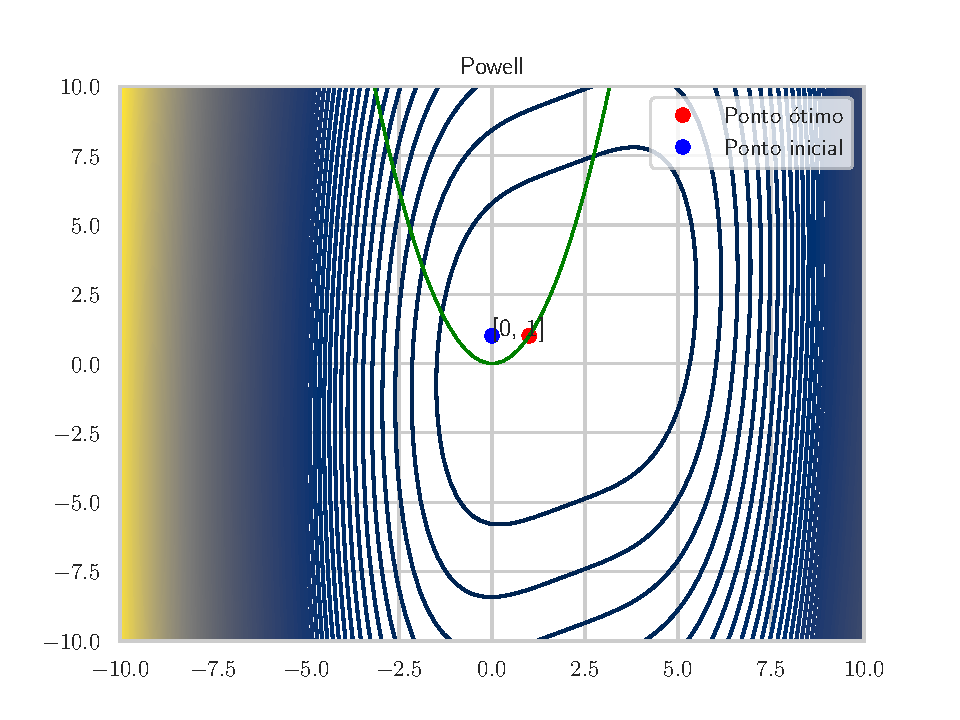
\includegraphics[scale = 0.6]{barreira_Powell_[0 1].pdf}
\end{figure}

\begin{figure}[H]
  \centering
  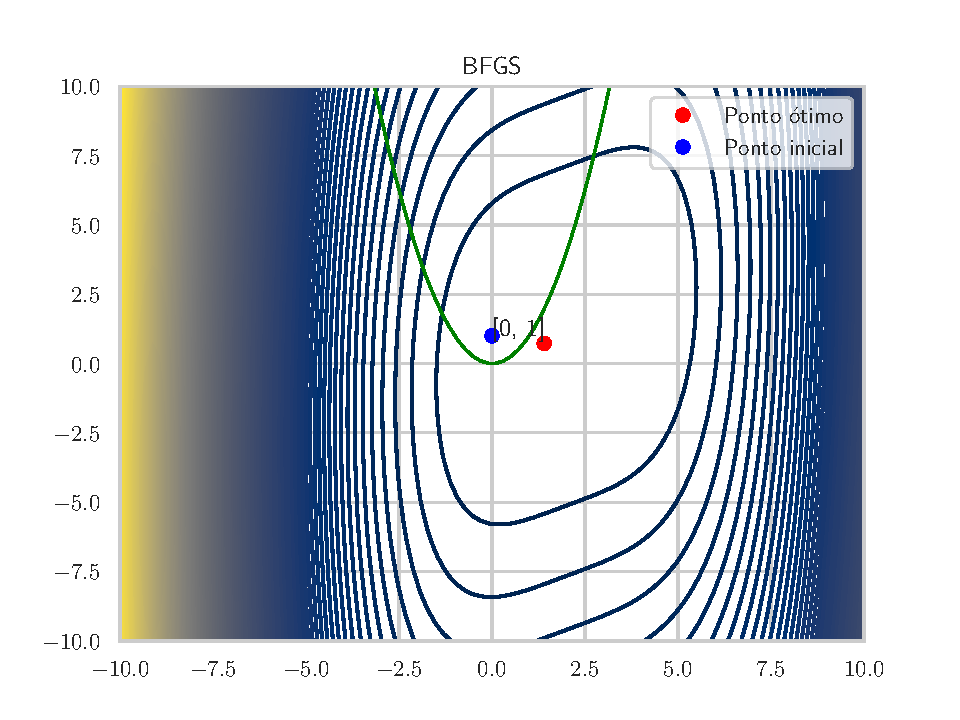
\includegraphics[scale = 0.6]{barreira_BFGS_[0 1].pdf}
\end{figure}

A tabela abaixo mostra que os métodos obtiveram resultados próximos.

\begin{table}[H]
\centering
\begin{tabular}{llr}
  \hline
  Método & x & f(x) \\
  \hline
  Powell & [1. 1.] & -inf \\
  BFGS & [1.40306585 0.72779351] & -0.676202 \\
  \hline
  \end{tabular}
\end{table}

\subsection{Problema 2}

\begin{equation}
  \begin{aligned}
      \text{Minimizar:} \quad & f(x_1, x_2) = -[(x_{1}+1)**2+(x_{2}+1)**2] \\
      \text{S.t:} \quad & x_1^2 + x_2^{2} - 2 \leq 0
  \end{aligned}
\end{equation}

Aplicando o método da \textbf{penalidade} para o problema proposto obtemos resultados para o método de Powell e para o método BFGS. Os gráficos abaixo apresentam as curvas de nível para a função objetivo e a penalidade (linha em verde). Além disso, é possível observar o ponto inicial e o ponto ótimo encontrado pelo algoritmo.

\begin{figure}[H]
  \centering
  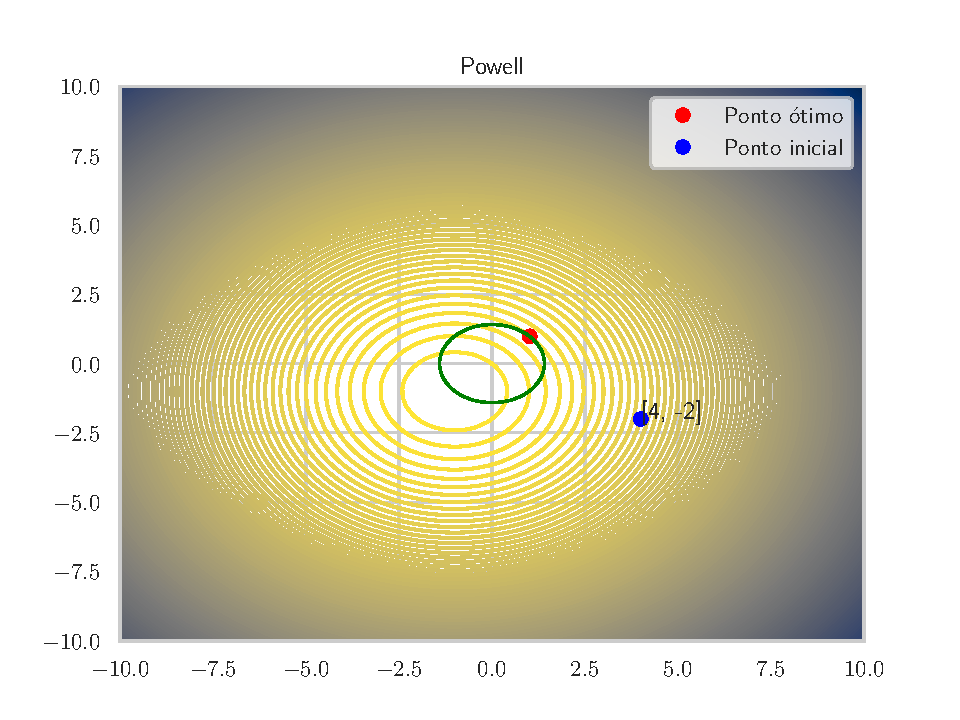
\includegraphics[scale = 0.6]{problema_2_penalidade_Powell_[ 4 -2].pdf}
\end{figure}

\begin{figure}[H]
  \centering
  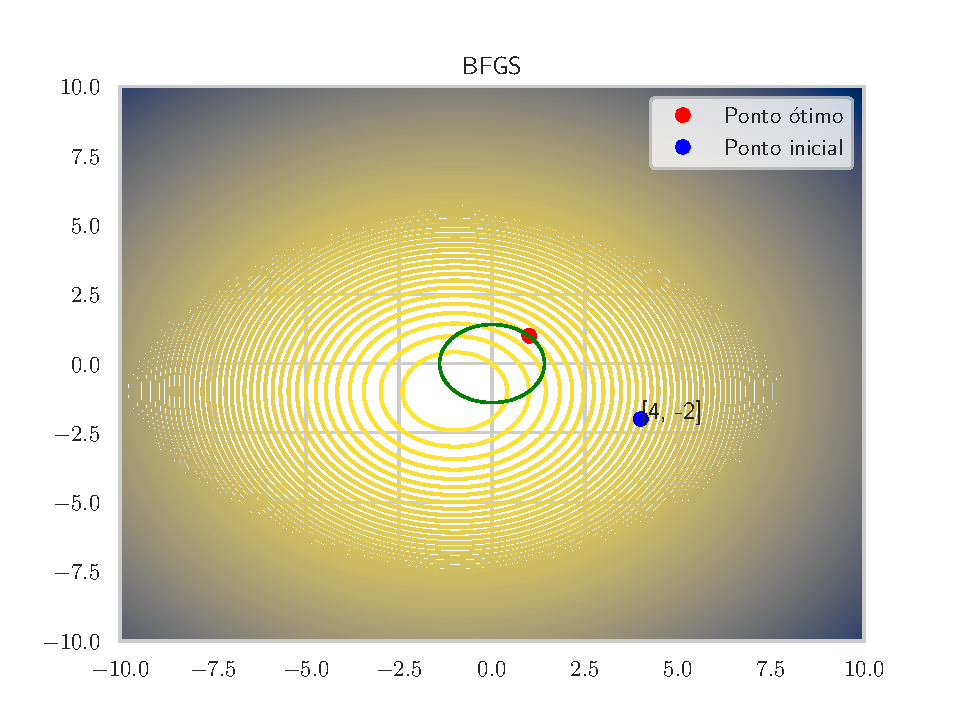
\includegraphics[scale = 0.6]{problema_2_penalidade_BFGS_[ 4 -2].pdf}
\end{figure}

A tabela abaixo mostra que os métodos obtiveram resultados próximos.

\begin{table}[H]
\centering
\begin{tabular}{llr}
  \hline
  Método & x & f(x) \\
  \hline
  Powell & [1.01428713 0.98550578] & -7.999586 \\
  BFGS & [0.99999644 1.00000356] & -8.000000 \\
  \hline
  \end{tabular}
\end{table}

Aplicando o método da \textbf{barreira} para o problema proposto obtemos resultados para o método de Powell e para o método BFGS. Os gráficos abaixo apresentam as curvas de nível para a função objetivo e a penalidade (linha em verde). Além disso, é possível observar o ponto inicial e o ponto ótimo encontrado pelo algoritmo.

\begin{figure}[H]
  \centering
  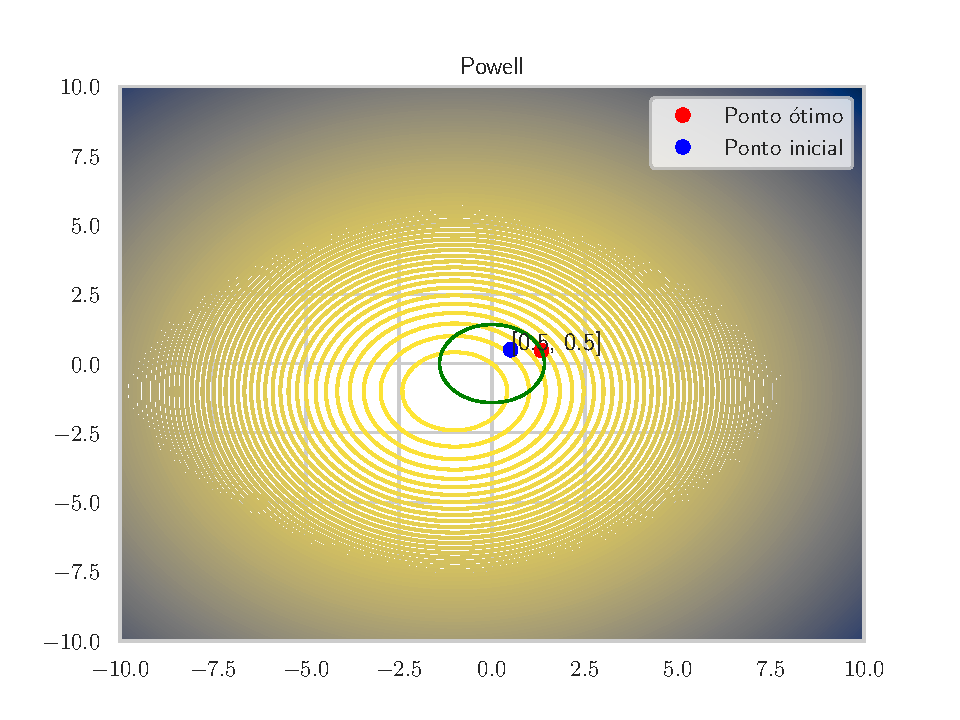
\includegraphics[scale = 0.6]{problema_2_barreira_Powell_[0.5 0.5].pdf}
\end{figure}

Observa-se que resultado para o método BFGS aplicando o método da barreira gerou um resultado incoerente com o observado no método de Powell. Nesse sentido, é preciso ainda realizar ajustes para que o método também funcione de maneira ótima.

\begin{figure}[H]
  \centering
  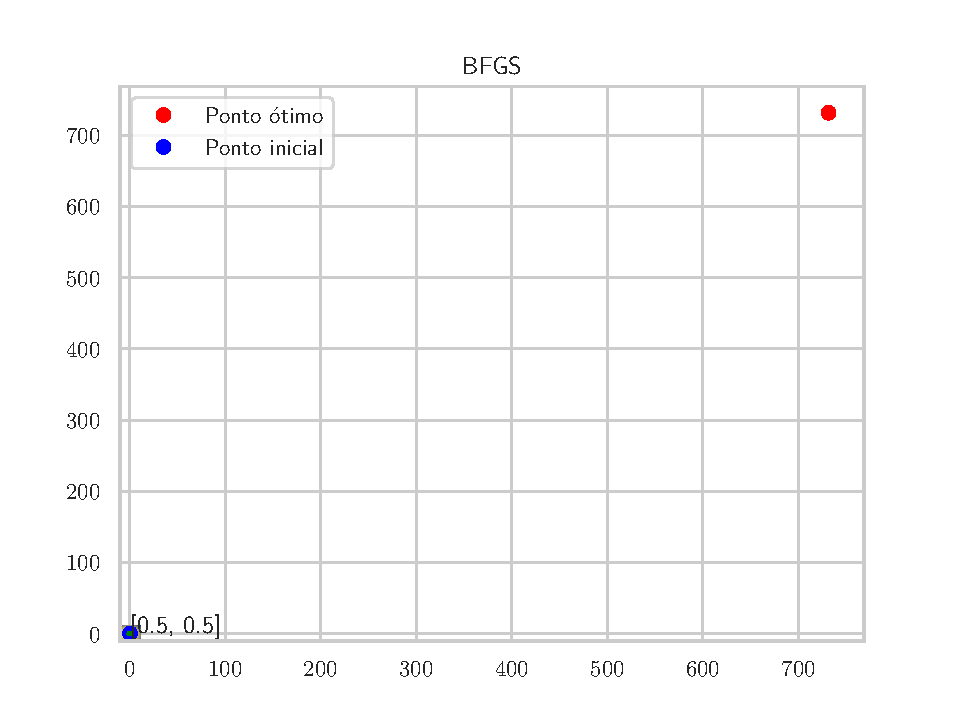
\includegraphics[scale = 0.6]{problema_2_barreira_BFGS_[0.5 0.5].pdf}
\end{figure}

A tabela abaixo mostra que os métodos obtiveram resultados próximos.

\begin{table}[H]
\centering
\begin{tabular}{llr}
  \hline
  Método & x & f(x) \\
  \hline
  Powell & [1.33239072 0.47406219] & -1804760610479.078613 \\
  BFGS & [731.71480095 731.71480095] & -1073741.959054 \\
  \hline
  \end{tabular}
\end{table}

\end{document}
